In this section, we will discuss the design-space of GPU-accelerated database systems. By exploring the design-space, we are trying to figure out the parameters on which we can survey and compare different database systems which support GPU acceleration. The outline of design-space with its corresponding parameters is shown in Figure \ref{fig:gpu_design_space}, on which we have surveyed different GPU-accelerated database systems in the later section.

\begin{figure}[ht]
\centering
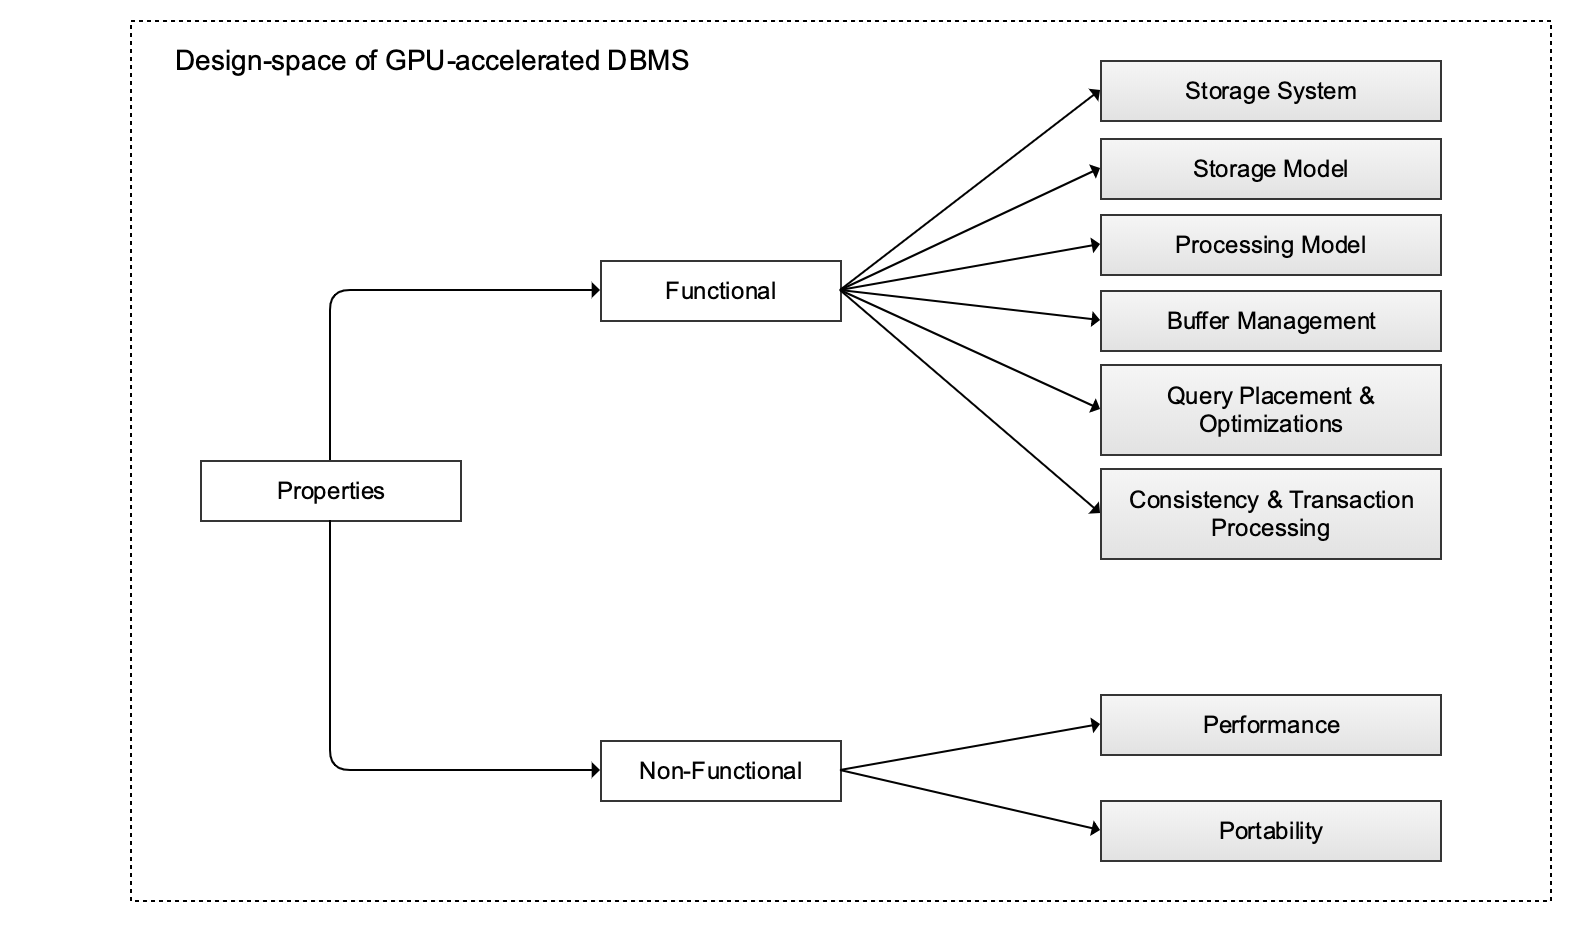
\includegraphics[width=\textwidth]{common/design_space}
\caption{The parameters of understanding GDBMS design-space}
\label{fig:gpu_design_space}
\end{figure}

\textbf{Functional Properties.} The properties which are comprised of understanding the functionalities of the system. These properties help us in providing the technical understanding of the workflows and give deep insight on how everything is managed in the system. After thorough research and analysis of the functional properties, we can deeply understands and survey how GPU-acceleration is being achieved by different database systems.

\textbf{Storage System.} A functional property which can be used to understand the underlying storage system of database systems with GPU-acceleration. In terms of the design-space, the storage system can describe the decision of GDBMS\footnote{GDBMS - GPU-accelerated database systems} of choosing a disk-based system or host's main-memory as their primary storage space.

\textbf{Storage Model.} After database system has decided which storage system will work as per their requirement, this property describes their decision of choosing how data is going to store in the selected storage system. These system can store their data in either row-store or column-store format.

\textbf{Processing Model.} This property describes the model adopted by the database system to process SQL queries. There are several processing models which are used in the database system widely such as tuple-at-a-time, operator-at-a-time, bulk-processing, record-oriented-processing and others. Depending upon the architectural implementation and requirements, GDBMS decide which processing model to choose and implement. 

\textbf{Buffer Management.} This property is used to describe the policies and strategies adopted by the GPU-accelerated database systems to manage data transfer requirements. Some system tends to create a specialized module while other manages it by implementing isolated programs which is usually executed on the host machine. Data transfer is an important requirement for these systems, due to the architectural design of the GPU.

\textbf{Query Placement and Optimizations.} This property is used to describe how optimizations are implemented in these database systems. Query placement describes scenarios where the system is able to decide which part of the query should be executed on which device in a multi-processing environment. Using this property, we can analyse the system's ability to perform automatic optimizations and fully utilise processing units in the system for maximum performance.

\textbf{Consistency and Transactions Processing.} This property is used to describe how the database system manages consistency and process transactions. It also analyzes the system's ability to perform and operate all transaction related operations such as commit, rollback and locking mechanisms such as 2-phase locking, optimistic locking and others. This parameter can help us to understand how fault tolerant is the system and the level of its consistency.
\newline

\textbf{Non-Functional Properties.} The properties which are used to understand non-functional aspects of the system. These properties are not used to describe system's technicalities and framework workflows. They are used to explain the overall system's operations, its identifiers and summarizing attributes and gives brief insights on the quality parameters.

\textbf{Performance.} This non-functional property helps us in reviewing the entire system's working and efficiency. It can describe the overall impact of the database system which can be compared with other similar systems for analyzing the implemented system's ability and throughput. We have used this property in our GDBMS survey to understand how much impact GPU-acceleration provide to the database system by comparing with CPU's main memory driven database systems.

\textbf{Portability.} This non-functional property is used to understand the system's ability to be independent of hardware requirements and specifications. It is used to analyse whether the database system is hardware-oblivious, independent of the hardware provided, or hardware-aware, dependent on the hardware specification. By reviewing the GPU-accelerated database system with this property, we can understand the dependencies and hardware requirements of the system, which is essential from the implementation perspective.

